\documentclass[11pt]{article}
\usepackage[margin=1in]{geometry}
\usepackage{graphicx}
\begin{document}
\section*{R92 independent rank-32 multiplication table}
The frozen R92 native run checked the unit and all 528 unordered basis
products. A fresh-readback, ideal-free F2(u) replay checked the full table,
16,896 polynomial coordinates and 528 corruption controls. A separate
source-field replay recomputed all 528 products. The exact post-run
comparison matched all 528 pair labels and 16,896 coefficients of the
previously accepted R50 table.

\begin{center}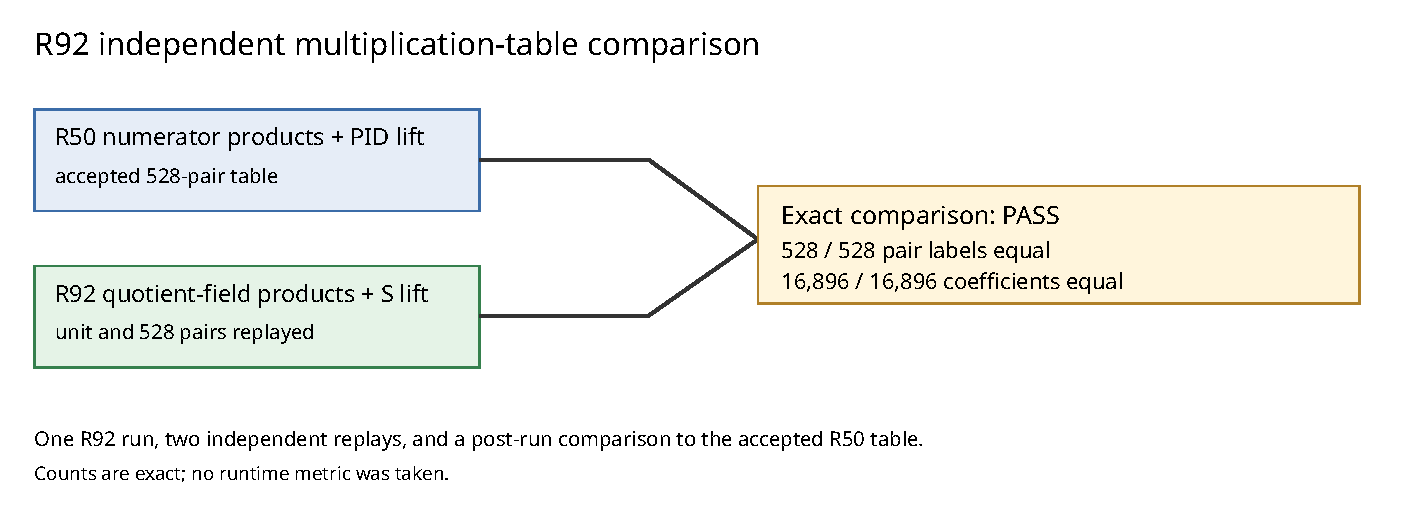
\includegraphics[width=\textwidth]{diagram.pdf}\end{center}

R50 had already established the table; R92 supplies a distinct
reconstruction and cross-check. Source revision:
\texttt{a58703742c8cdd4a91beb0eb1bc78c7eb8cb0c51}. The one-thread
Singular/FLINT run used seed 92, a 4 GiB virtual-memory cap and a
1200-second timeout. All 18 raw members passed fresh-readback hashes.
The next task is explicit chart gluing and proper boundary checks,
then the modular-factor action. See \texttt{CM.md} and
\texttt{SCOPE-ERRATUM.md} for the claim boundary.
\end{document}
